\documentclass{article}

%\usepackage[space]{xeCJK}
\usepackage[hyphens]{url}
\usepackage{listings}
\usepackage[a4paper,top=3cm,bottom=2cm,left=3cm,right=3cm,marginparwidth=1.75cm]{geometry}
\usepackage{xcolor}
\usepackage{lscape}
\usepackage{pdflscape}
\usepackage{natbib}
\usepackage{graphicx}  
\usepackage[colorlinks, citecolor=red]{hyperref}
\usepackage{caption}
\usepackage{float}
\usepackage{graphicx, subfig}
\usepackage{ulem}

\title{Yu-Lab Weekly Report (Update)}
\newcommand\todo[1]{\textcolor{red}{#1}}

\begin{document}
\author{Haojun Li}
\maketitle

\section{Introduction}

\subsection{Background}
In tumor microenvironment, the cellular composition of the immune infiltrate of tumors can shed light on the escape mechanisms that tumor cell use to evade the immune response. In clinical trials, it can be used to stratify patients to assign most suitable treatment options depending on the targeted cell type, hence increasing the overall chances of success, and ultimately accelerating access to improved treatment options. Changes in tissue composition are often indicative of disease progression or drug response. As interactions between the immune system and tumour cells are governed by a complex network of cell–cell interactions, especially, knowing the specific immune cell composition of a solid tumour may be essential to predict a patient's response to immunotherapy~\cite{Schelker2017Estimation}. 

With the development of gene sequencing technology, the investigation of the causes and treatment effects of diseases has become more available. Gene expression profiling, RNA-seq and mircoarray has been optimized to be applicable in clinical.

In the past, Fluorescence Activated Cell Sorting (FACS), Immunohistochemistry (IHC) and Immuno Fluorescence (IF) which utilize only a small number of cell type specific markers was used to measure the components in a mixed patient sample. In recent years, more and more biologists use single cell RNA-seq to calculate the cellular composition of a mixed tissue or sample to explore the pathogenic mechanism and therapeutic methods, especially in complex tissue samples, such as tumor tissues. In single cell RNA-seq, individual cells from a mixed sample are labeled and sequenced, and cell components in tissue are determined by grouping and clustering. Both FACS and single cell RNA-seq not only involve significant time, effort, and expense but also result in insufficient RNA abundance for further quantification of gene expression in some cases.

Deconvolution is the method of estimating individual signal components from their mixtures in the area of signal processing. It has diverse applications in fields ranging from hyperspectral imaging to noise cancellation in audio recordings. In the field of biomedical research, we can use this method to estimate the cellular specific components in complex tissues in order to identify the changes in cellular components in tissues. Deconvolving data from biopsy tissues allows further investigation of the interaction between tumor and micro-environmental cells, and role of such interaction in the progression of cancer.

At least seven major issues raise concerns that the \textit{in silico} methods could be prone to errors and cannot reliably portray the cellular heterogeneity of the tumor microenvironment. The main issues are as follows.
\begin{itemize}
    \item Current techniques depend on the expression profiles of purified cell types to identify reference genes and therefore rely heavily on the data source from which the references are inferred and could this be inclined to overfit these data. 
     \item Current methods focus on only a very narrow range of the tumor microenvironment, usually a subset of immune cell types, and thus do not account for the further richness of cell types in the microenvironment, including blood vessels and other different forms of cell subsets.
      \item The ability of cancer cells to “imitate” other cell types by expressing immune-specific genes, such as a macrophage-like expression pattern in tumors with parainflammation; only a few of the methods take this into account. 
       \item The ability of existing methods to estimate cell abundance has not yet been comprehensively validated in mixed samples. Cytometry is a common method for counting cell types in a mixture and, when performed in combination with gene expression profiling, can allow validation of the estimations. However, in most studies that include cytometry validation, these analyses were performed on only a very limited number of cell types and a limited number of samples. 
        \item Deconvolution approaches are prone to many different biases because of the strict dependencies among all cell types that are inferred. This could highly affect reliability when analyzing tumor samples, which are prone to form non-conventional expression profiles. 
         \item Deconvolution infers an increasing number of closely related cell types.
          \item Deconvolution analysis heavily relies on the structure of the reference matrix, which limits its application to the resource used to develop the matrix.
\end{itemize}

\subsection{Prior Art}

\subsubsection{2019.4.3}
(1) This paper~\cite{Danaher2017} uses co-expression patterns in large tumor gene expression datasets to evaluate previously reported candidate cell type marker genes lists, eliminate numerous false positives and identify a subset of high confidence marker genes. The main contributions of this paper include 1) identify a list of 60 marker genes whose expression levels measure 14 immune cell populations; 2) most genes previously reported to be enriched in a single cell type have co-expression patterns inconsistent with cell type specificity. The main disadvantages of this paper include 1) many cell types are short of markers such as CD4 T cell, Monocytes.

\subsubsection{2019.3.2}
(1) This paper~\cite{Sturm463828} presents a systematic approach for benchmarking such computational methods and assessed the accuracy of tools at estimating nine different immune and stromal cells from bulk RNA-seq samples. The main contributions of this paper include 1) collecting an amount of single cell RNA-seq data set; 2) Benchmark methods performance between cell types, background predictions and spillover to give a guidelines for method selection.

(2) This paper~\cite{Finotello2018Quantifying} describes the state-of-the-art computational methods for the quantification of immune cells from transcriptomics data and discuss the open challenges that must be addressed to accurately quantify immune infiltrates from RNA sequencing data of human bulk tumors. This review makes a detailed classification and induction of the current deconvolution methods.

\subsubsection{2019.2.25}
(1) This paper~\cite{Vallania206466} presents immunoStates, a basis matrix built using 6160 samples with different disease states across 42 microarray platforms. The main contributions of this paper include 1) it found that deconvolution accuracy is more dependent on the signature matrix through experiments; 2) they create immunoStates which significantly reduces biological and technical biases by using healthy and disease samples and Hedeg's g effect sizes; 3) This matrix has leads to better deconvolution performance than LM22 and IRIS, independent of the deconvolution algorithms tested.

(2) This paper~\cite{Nirmal1388} presents ImSig from tissue transcriptomics data using a network-based deconvolution approach. The main contributions of this paper include 1) it used tissue sample which can reflect the differentiation or activation state of similar cells within tissues; 2) they used gene correlation network, Markov clustering alforithm (MCL), Gene Ontology (GO) in signature creating. The main disadvantage of this paper is the lack of performance comparison of this signature matrix with other common feature matrices such as LM22 and IRIS.

(3) This paper~\cite{Chen2018} introduced a method called MySort, using microarray data from the public domain to profile gene expression pattern of twenty-two immune cell types. MySort is an improvement over CIBERSORT with a few additional steps and changes in the pipline. The main contributions of this paper include 1) using enrichment score (ES), two-sided unequal variance T-test and differentially expressed genes (DEGs) to define signature matrix; 2) it added clustering, pearson correlation to remove outliers based on CIBERSORT deconvolution pipeline. The main disadvantage of this paper is the lack of performance comparison with other methods.

\subsubsection{2018.12.21}
This paper~\cite{Etienne2016Estimating} introduced a method called Microenvironment Cell Populations-counter (MCP-counter), which allows the robust quantification of the absolute abundance of eight immune and two stromal cell populations in heterogeneous tissues from transcriptomic data. The main contributions of this paper include 1) the paper has detailed the cell type classification and collection of purified cell data; 2) This method screens the marker for specific cell types. The main disadvantages of this paper include 1) the algorithm has no feature matrix, but only judges the expression of the selected marker; 2) MCP-counter score cannot represent the actual fraction. 

\subsubsection{2018.11.23}
This paper~\cite{Aran2017xCell} introduced a method called xCell, a novel gene signature-based method, and use it to infer 64 immune and stromal cell types. The main contributions of this paper include 1) collecting the most comprehensive resource to date of primary cell types, spanning the largest set of human cell types; 2) gene signatures are rank-based and are therefore suitable for cross-platform transcriptome measurements. The main disadvantages of this paper include 1) the inferences are strictly enrichment scores, and cannot be interpreted as proportions because of the inability to translate the minimum and maximum scores produced by ssGSEA to clear proportions and 2) Expression of purified cell types measured from different tissues may be different.

\subsubsection{2018.11.09}
(1) This paper~\cite{Hao358366} introduced a method called FARDEEP utilizing an adaptive least trimmed square to automatically dectet and removing outliers before estimating the cell compositions. The main contributions of this paper include 1) evaluates all outliers across the datasets and 2) examining the true immune gene signature using non-negative regression and 3) improving prognostic potential when dealing more complex datasets with significant carcinoma cell content. This method has compared with other method including NNLS, PERT~\cite{Qiao2012PERT}, DCQ~\cite{Altboum2014Digital}, CIBERSORT~\cite{Newman2015Robust}. But its Performance criteria are sum of squared error(SSE) and codfdicient of determination denoted as R-square. Especially, FAEDEEP has better performance than CIBERSORT through SSE and R-square. But CIBERSORT used RMSE and R to evaluate performance, and the review~\cite{Mohammadi2017A} selects MSE. Different performance criteria will affect the performance comparsion.

(2) This paper~\cite{Newman2016High} discusses the application of Deconvolution in Tumor infiltrating leukocytes (TILs). The main contributions of this paper include 1) Comparing and summarizing the functions of existing deconvolution methods in TILs and 2) Discussing the more significant problems at present.

\subsubsection{2018.11.02}
(1) This paper~\cite{Lehmusvaara2010Probabilistic} introduced a method called Dsection based on probability model. The main contributions of this paper include 1) de-noising uncertain prior information about cell-type proportions and 2) Use prior knowledge to ensure the accuracy of prediction. The shortcoming of this paper is that the number of cell types need to be known.

(2) This paper~\cite{Li2017Revisit} thinks that CIBERSORT~\cite{Newman2015Robust} actually has more errors including 1) considering the significant impact of data normalization on deconvolution results, and nonbiological negative correlations mainly due to collinearity in CIBERSORT, 2) using flow cytometry experiment to argue that closely related immune cell types should be positively correlated in abundance, whether in blood or in tumors, 3) claiming that up to 25 percent of LM22 genes are positively correlated with tumor purity.   

(3) This paper~\cite{Newman2017Data} responds to accusations and gives explanations to another paper~\cite{Li2017Revisit} including 1) TIMER mixed populations do not sum to 100 percent and are therefore unsuitable for addressing this topic, 2) no significant association between pairwise correlations of leukocyte estimates in tumors and pairwise correlations of corresponding expression profiles in LM22, 3) claiming that exclusion of all significantly positively correlated genes from LM22 had virtually no impact on tumor deconvolution performance.   

\subsubsection{2018.10.28}
I prepare for the presention based on the paper~\cite{Mohammadi2017A}, review of deconvolution, the Related method like LLSR~\cite{Abbas2009Deconvolution}, QP~\cite{Gong2011Optimal}, CIBERSORT~\cite{Newman2015Robust}, DSA, TIMER and so on. What's more, I summarized six points that may improve the doconvolution performance in the future.

\subsubsection{2018.10.19}
(1) This paper ``ML Estimation of Cell Fraction'' introduced a method for ML estimation.The main contributions of this paper include 1) Applying decoding from channel coding to Deconvolution and 2) Use prior knowledge to ensure the accuracy of prediction.

(2) This paper~\cite{Gong2011Optimal} introduced a method for quadratic programming. The main contributions of this paper include 1) buliding a system of linear equations through the introduction of a least squares and 2) the explicit modeling of physical constraints in both the description of the problem as well as its solution and 3) suggesting we can only apply on specific tissue to gain the best performance.

\subsubsection{2018.10.12}
I configure the environment and install CIBERSORT~\cite{Newman2015Robust} on Ubuntu. I try to run GSE11103, mixtures of four blood cell line. And I also try to run the GEPs from paper of Global characterization of T cells in non-small-cell lung cancer by single-cell sequencing, but errors occur. I think it may due to the format of data. On the other hand, I read the CIBERSORT online method and supplementary in order to find it how to evaluation its performance and compare with other methods. CIBERSORT use Pearson correlation and r.m.s. error to measure linear fit and estimation bias. It also simulates tumors with added noise and cell subset detection limit to compare with other method. But the main problem is the data need to combine two GEPs, but they don't provide the detail methods.

\section{Method}
\subsection{Data preparation}

\subsubsection{Cancer cell expression profiles}
I downloaded about 500 sample LUAD RNA-Seq expression profiles from \href{https://portal.gdc.cancer.gov/}{TCGA}.
I transformed ensembl id into gene, transformed FPKM format into TPM, removed nulls and duplicates with R code, finally sort TCGA data into available expression profiles.

\subsubsection{Purity cell expression profiles}

(1) I downloaded the RNA-Seq purified cell matrix including SRR1740038, SRR1740039, SRR1740040, SRR1740041, SRR1740066, SRR1740067, SRR1740068, SRR1740069 in \href{https://www.encodeproject.org/}{ENCODE project} following the paper~\cite{Aran2017xCell}.

(2) I downloaded the microarray purified cell matrix in \href{https://www.ncbi.nlm.nih.gov/geo/}{GEO} with cel format following the paper~\cite{Etienne2016Estimating}.

10 cell types were selected  which have a enough amount of purified expression samples including B cells, CD4 T cells, CD8 T cells, NK cells, Dendritic cells, Neutrophils, Monocytes, fibroblast, Macrophages, Endothelium. I collected each cell type purified samples from microarray as follow.

\begin{enumerate}
     \item B cell are from GSE22886, GSE43677, GSE9378, GSE54017, GSE13411, GSE12845, GSE18723, above 125 sample.
     \item CD4 T cell are from GSE22886, GSE2270, GSE8835, GSE7497, GSE36476, GSE20198, GSE13017, GSE17354, above 164 samples.
     \item CD8 T cell are from GSE22886, GSE8835, GSE11188, GSE17354, above 44 samples.
     \item Endothelium are from GSE9378, GSE9877, GSE32710, GSE22688, GSE14230, above 116 samples.
     \item Fibroblast are from GSE40839, GSE30242, above 45 samples.
     \item Macrophages are from GSE16972, GSE22528, GSE5099, GSE9874, GSE49072, GSE8515, above 158 samples.
     \item Monocytes are from GSE22886, GSE8921, GSE16972, GSE9378, GSE11943, GSE5099, GSE12837, GSE46923, above 170 samples.
     \item Myeloid Dendritic Cells are from GSE22886, GSE12259, GSE14816, GSE9946, GSE46923, above 44 samples.
     \item Neutrophils are from GSE22886, GSE12837, GSE19556, GSE12484, above 18 samples.
     \item NK cells are from GSE22886, above 15 samples.
\end{enumerate}
\begin{figure}[H]
     \centering
     \includegraphics[width=5in]{pic/celltype.jpeg}
     \caption{Cell type classification pyramidal graph}
     \label{fig:f1}
\end{figure}

\subsubsection{True mixture expression profiles with konwn fraction}
I downloaded GSE64385 from GEO~\cite{Etienne2016Estimating} to gain In vitro RNA mixtures. The dataset is microarray data in Affymetrix Human Genome 133 Plus 2.0 Gene expression platform including 12 mixtures sample and 5 immune cell with known fraction. 5 immune cell populations were sorted from 3 healthy donors' peripheral bloods. Peripheral Blood Mononuclear Cells (PBCMs) and PolymorphoNuclear Cells (PMN) were separated using gradient centrifugation. T cells (DAPI-/CD3+/CD14-/CD19-/CD56-), monocytes (DAPI-/CD3-/CD14+/CD19-/CD56-), B cells (DAPI-/CD3-/CD14-/CD19+/CD56-) and NK cells (DAPI-/CD3-/CD14-/CD19-/CD56+) were FACS-sorted from PBMCs and neutrophils (DAPI-/CD66b+/CD19-/CD3-/CD56-/CD14-) were sorted from PMNs. RNA was extracted from the purified cell population, as well as from the HCT116 colon cancer cell line. RNAs from pure populations were then mixed in various proportions.

\subsection{Mixture simulating and marker gene selecting}
(1) I used ReadAffy function in R code to read purified cel format microarray data, then standardize it with rma. For subsequent mixing, I made a power to its expression value. 

\subsection{Algorithm implementation}
\subsubsection{Supervised learning - mult-output regression}
\begin{figure}[H]
     \centering
     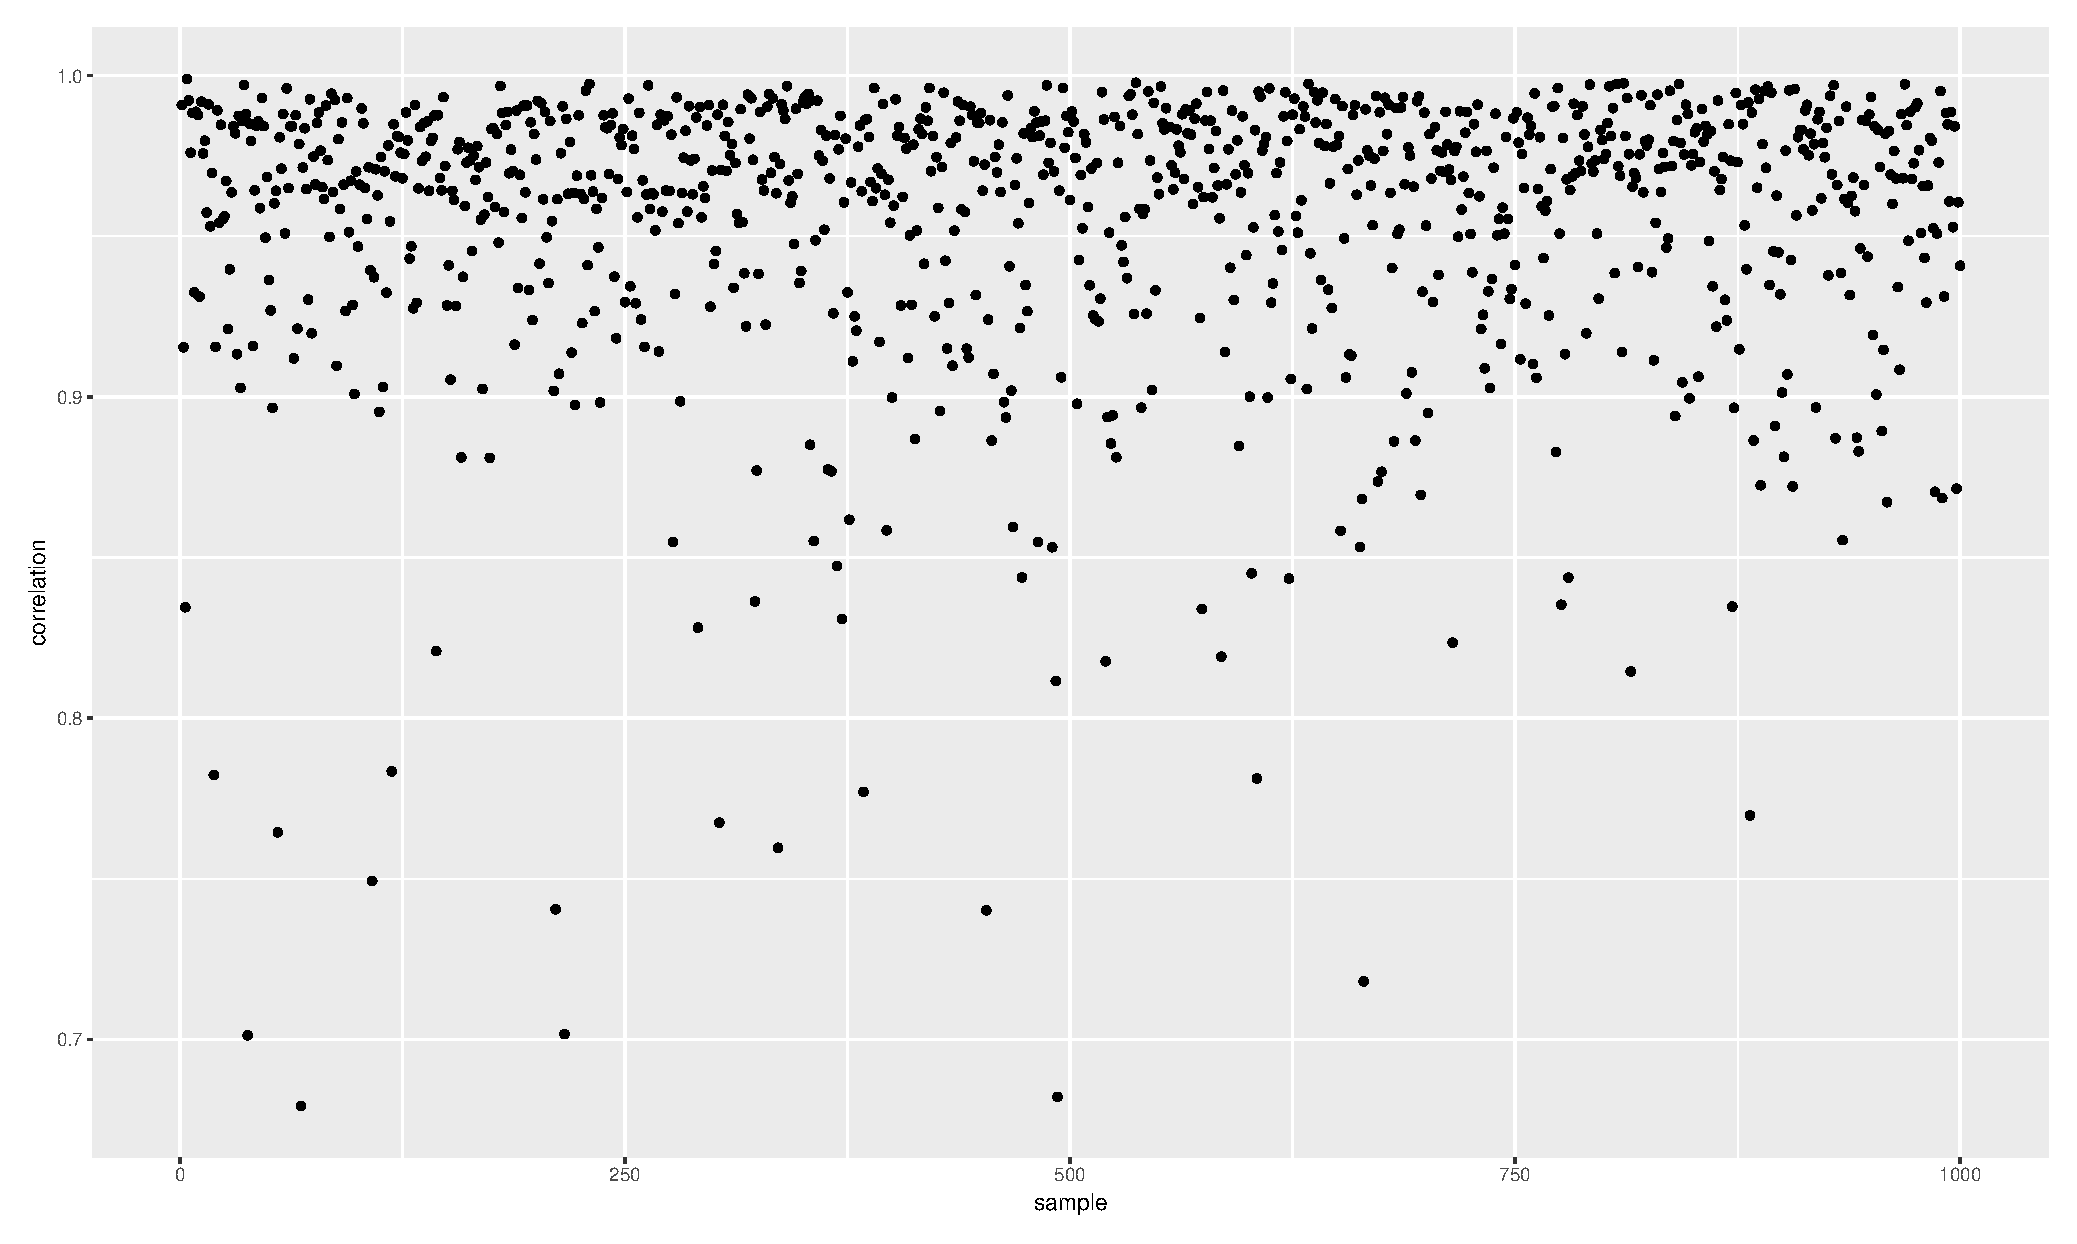
\includegraphics[width=5in]{pic/morden_corr1000.eps}
     \caption{correlation between predicted an true fraction}
     \label{fig:f2}
\end{figure}

\subsection{Suggestion}
Possible ways to improve the deconvolution are as follows:
\begin{enumerate}
\item Different methods have different performance on different data, so the method need requires a corresponding prior knowledge of different data~\cite{Qiao2012PERT}~\cite{Liebner2014MMAD}~\cite{Lehmusvaara2010Probabilistic}. 

\item Explicit STO can cause lower performance of deconvolution, so the method of filtering violating feature need to be improved~\cite{Mohammadi2017A}.

\item Different upper/lower bounds have been proposed in the literature to prefilter expression values prior to deconvolution. Filter lower and upper bounds of gene expressions using adaptive range filtering may improve deconvolution performance\cite{Mohammadi2017A}.

\item Select invariant (among references and between references and samples) cell-type-specific markers to enhance the discriminating power of the basis matrix~\cite{Mohammadi2017A}~\cite{Newman2015Robust}~\cite{Yi2013Digital}~\cite{Liebner2014MMAD}.

\item Solve the regression using the L2 loss function together with an R2 regularizer, or group LASSO if sparsity is desired among groups of tissues/cell types~\cite{Mohammadi2017A}~\cite{Newman2015Robust}.

\item For tumor cells, construct a purification characteristic matrix corresponding to tumor malignant cells, or perform prior probability statistics on the purity of tumor cells to improve the accuracy of deconvolution~\cite{Yi2013Digital}\cite{Bo2016Comprehensive}.

\item We should consider the performance criteria.
\end{enumerate}


\section{Simulations and results}

\subsection{Purired RNA-seq Data}
 Dendritic cells RNA-seq TPM data from Quantiseq dataset, sequenced by Quantiseq.

 \begin{figure}[H]
     \centering
     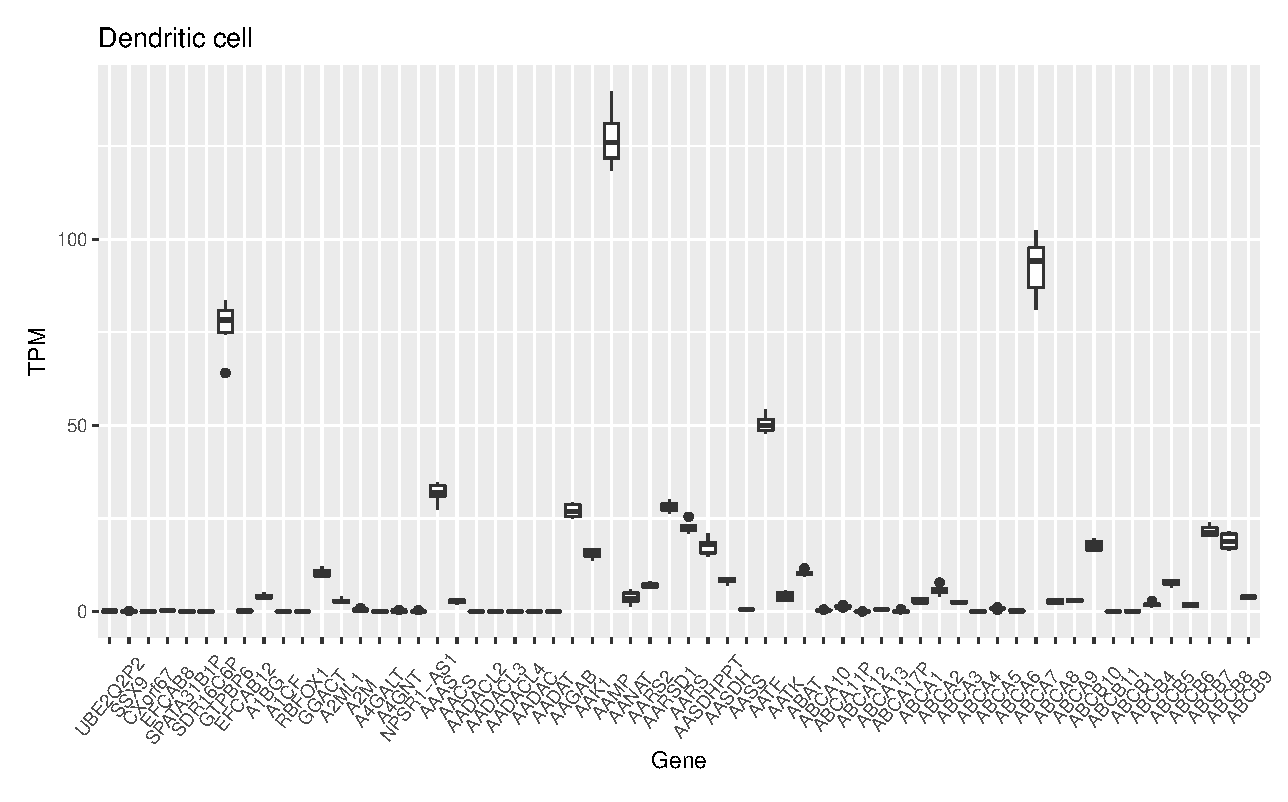
\includegraphics[width=5in]{Dendritic_cell_50.eps}
     \caption{Dendritic cells TPM distribution }
     \label{fig:my_label}
 \end{figure}
 
 \subsection{Purified Microarray Data }
 Data are from GSE473, GSE6740, GSE13017, GSE17354, including 118 samples in order to explore microarray CD4 T cells expression distribution.
 Different genes in CD4 T cells are clearly distributed in cell expression.

\begin{figure}[H]
     \centering
     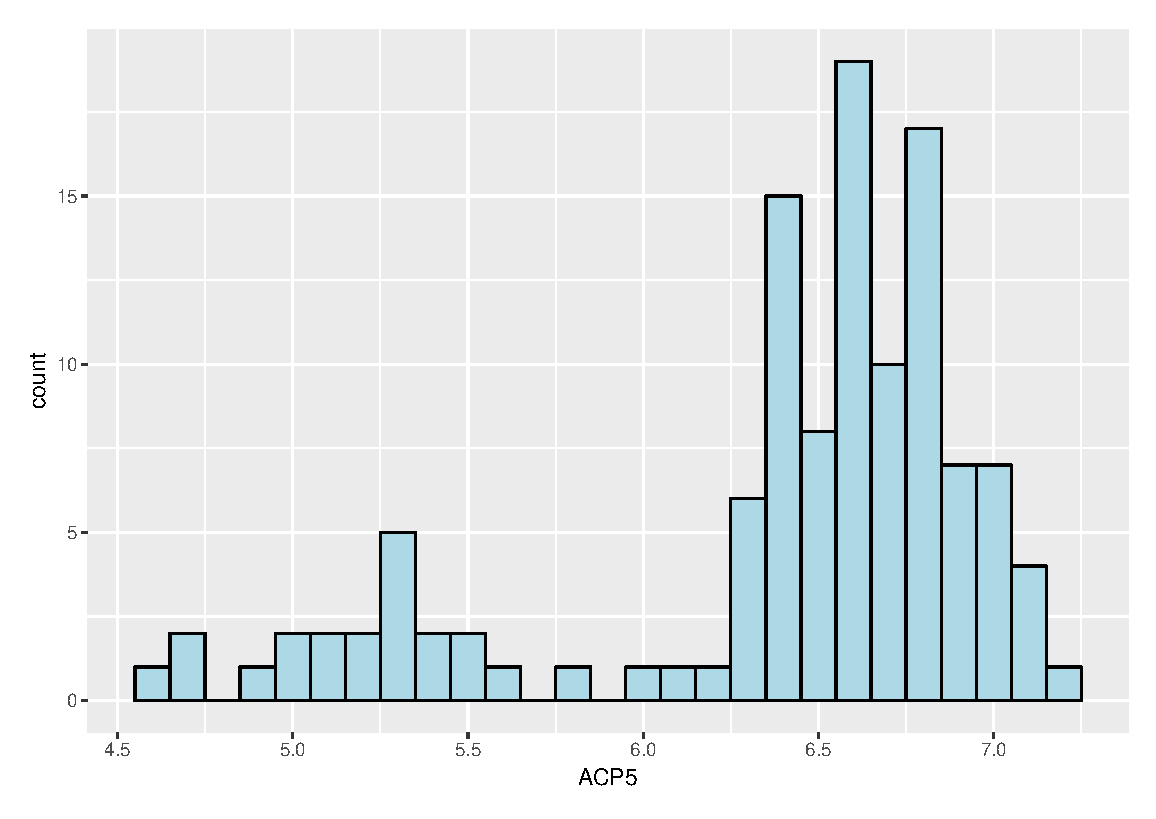
\includegraphics[width=5in]{CD4T_ACP5_log.eps}
     \caption{CD4 T cells ACP5}
     \label{fig:my_label}
\end{figure}
 
\begin{figure}[H]
     \centering
     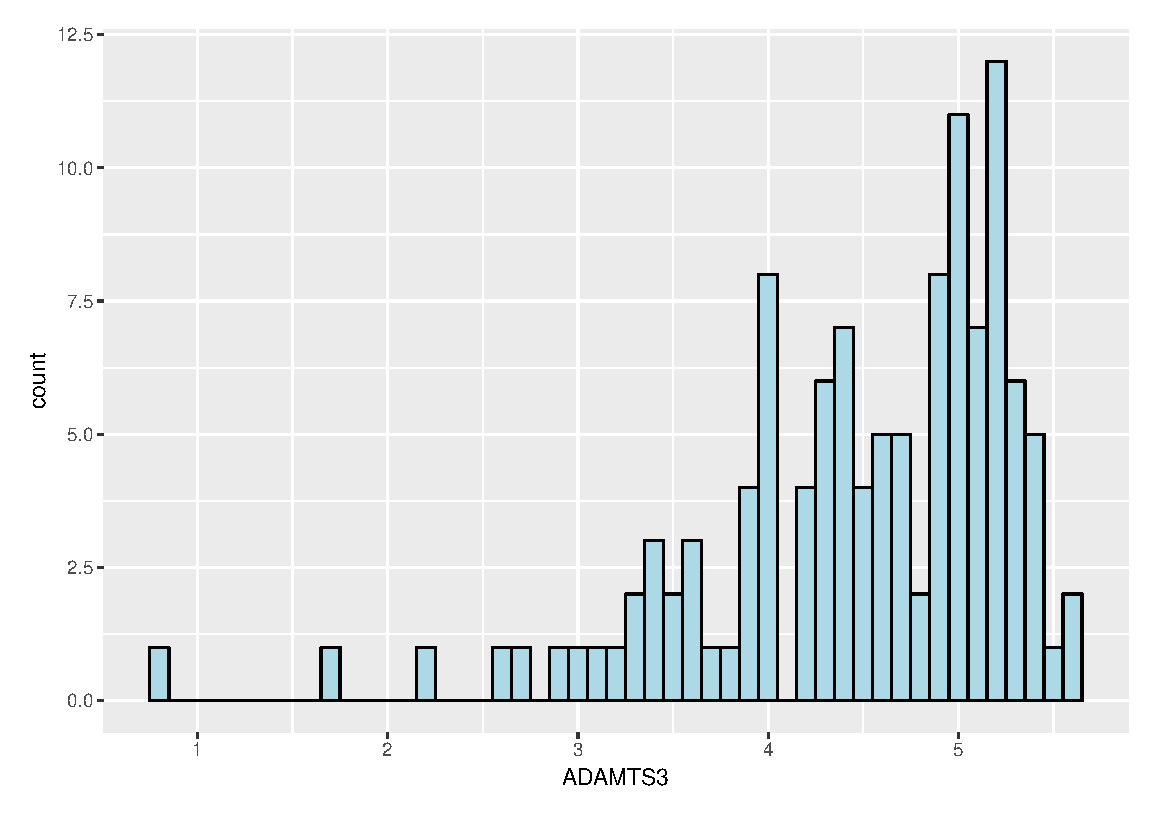
\includegraphics[width=5in]{CD4T_ADAMDEC1_log.eps}
     \caption{CD4 T cells ADAMDEC1}
     \label{fig:my_label}
\end{figure}
\begin{figure}[H]
     \centering
     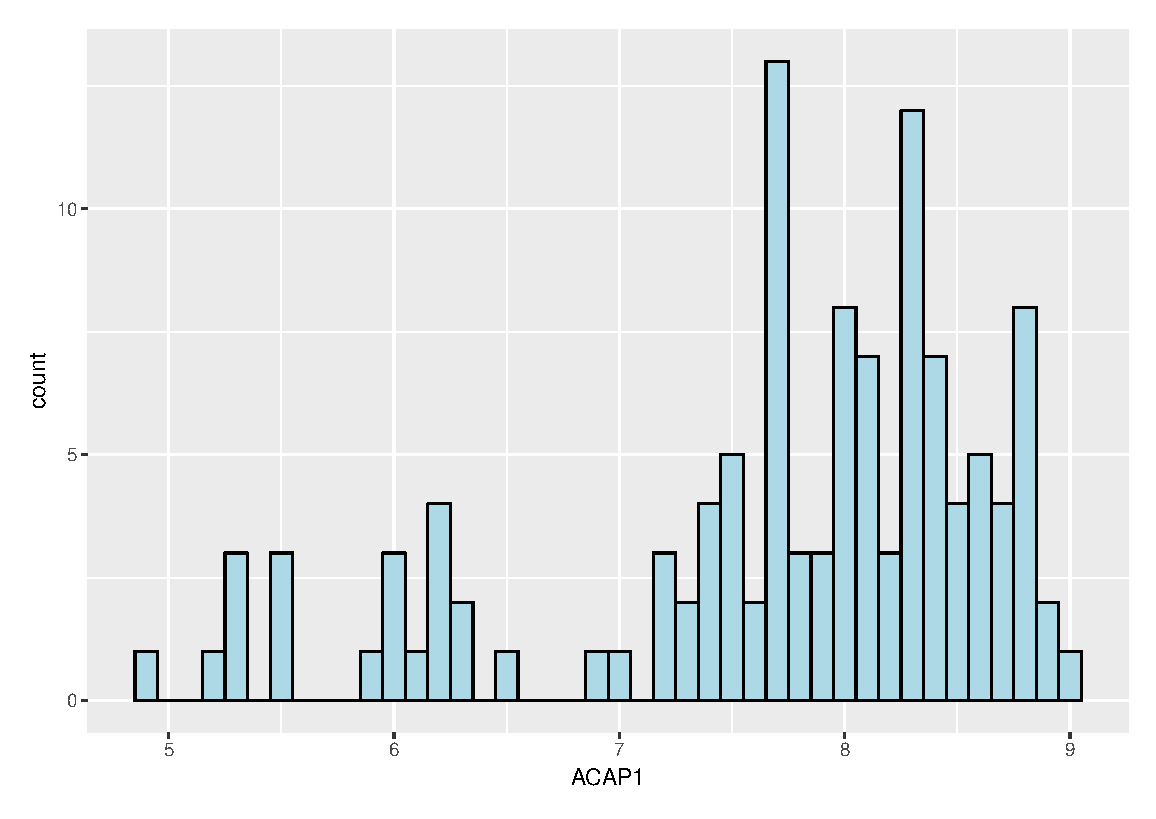
\includegraphics[width=5in]{pic/CD4T_ACAP1_log.eps}
     \caption{CD4 T  cells ACAP1}
     \label{fig:my_label}
\end{figure}
\begin{figure}[H]
     \centering
     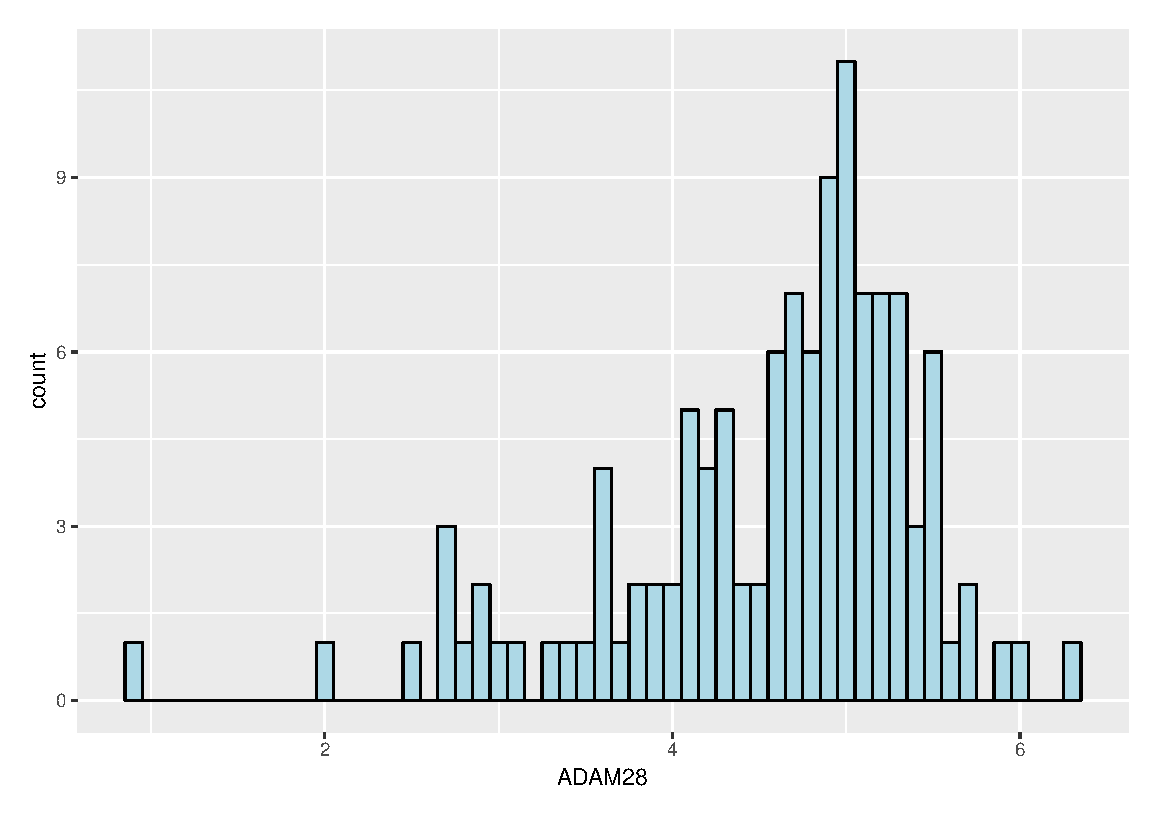
\includegraphics[width=5in]{CD4T_ADAM28_log.eps}
     \caption{CD4 T cells ADAM28}
     \label{fig:my_label}
\end{figure}
\begin{figure}[H]
     \centering
     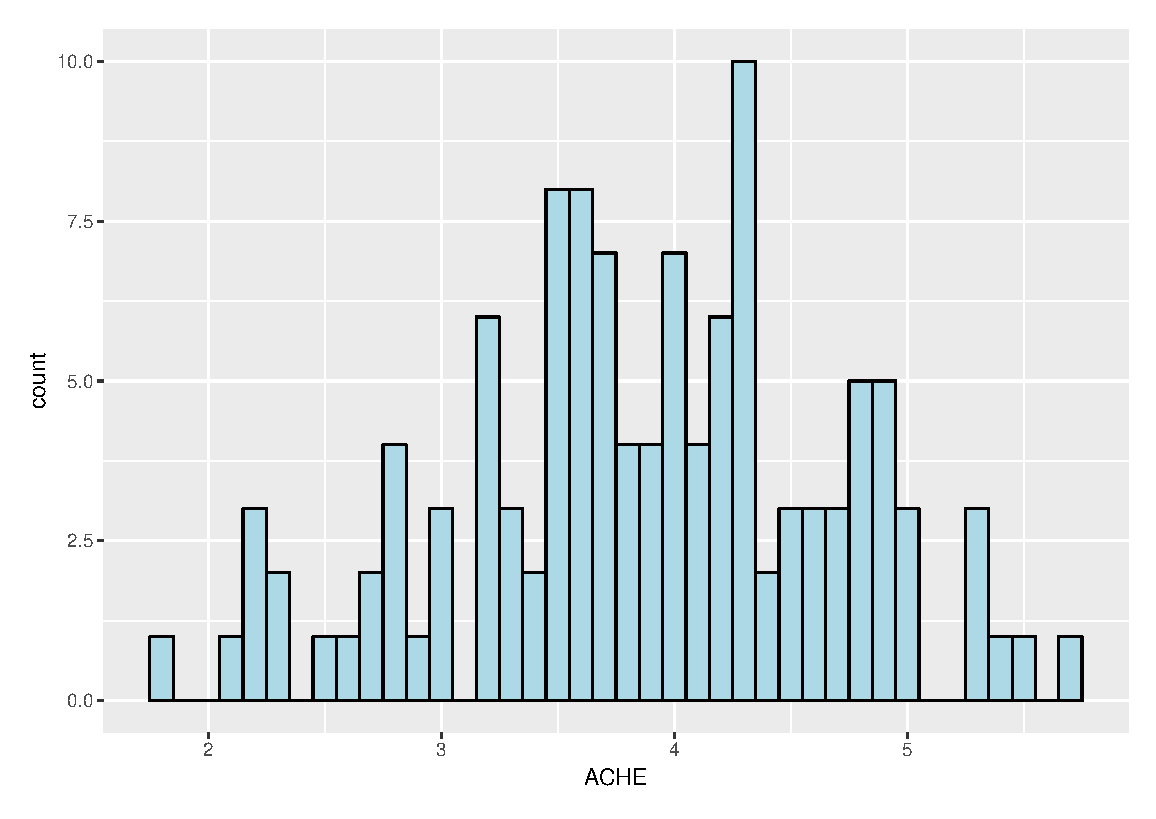
\includegraphics[width=5in]{CD4T_ACHE_log.eps}
     \caption{CD4 T cells ACHE}
     \label{fig:my_label}
\end{figure}
 
  \subsection{MCP-count test}
  I downloaded cel format Micoarray data from GSE22886. Six cell types were selected including B cell, CD8 T cell, NK cell, Myeloid dendritic cell, Monocytes, Neutrophils. I mixed them with random fraction, and ran MCP-count with them.
  \begin{figure}[H]
     \centering
     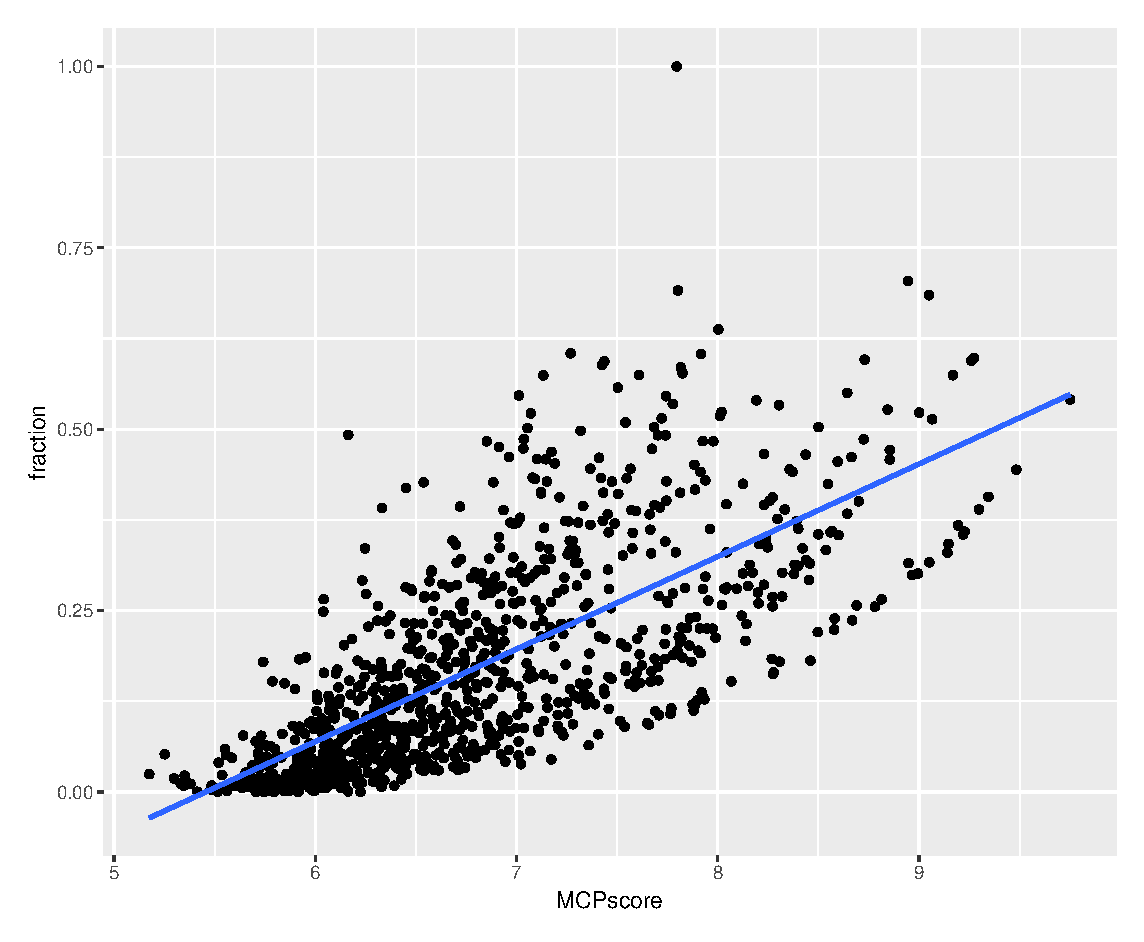
\includegraphics[width=5in]{MCP-CD8T.eps}
     \caption{MCP-count CD8 T cell}
     \label{fig:my_label}
 \end{figure}
 \begin{figure}[H]
     \centering
     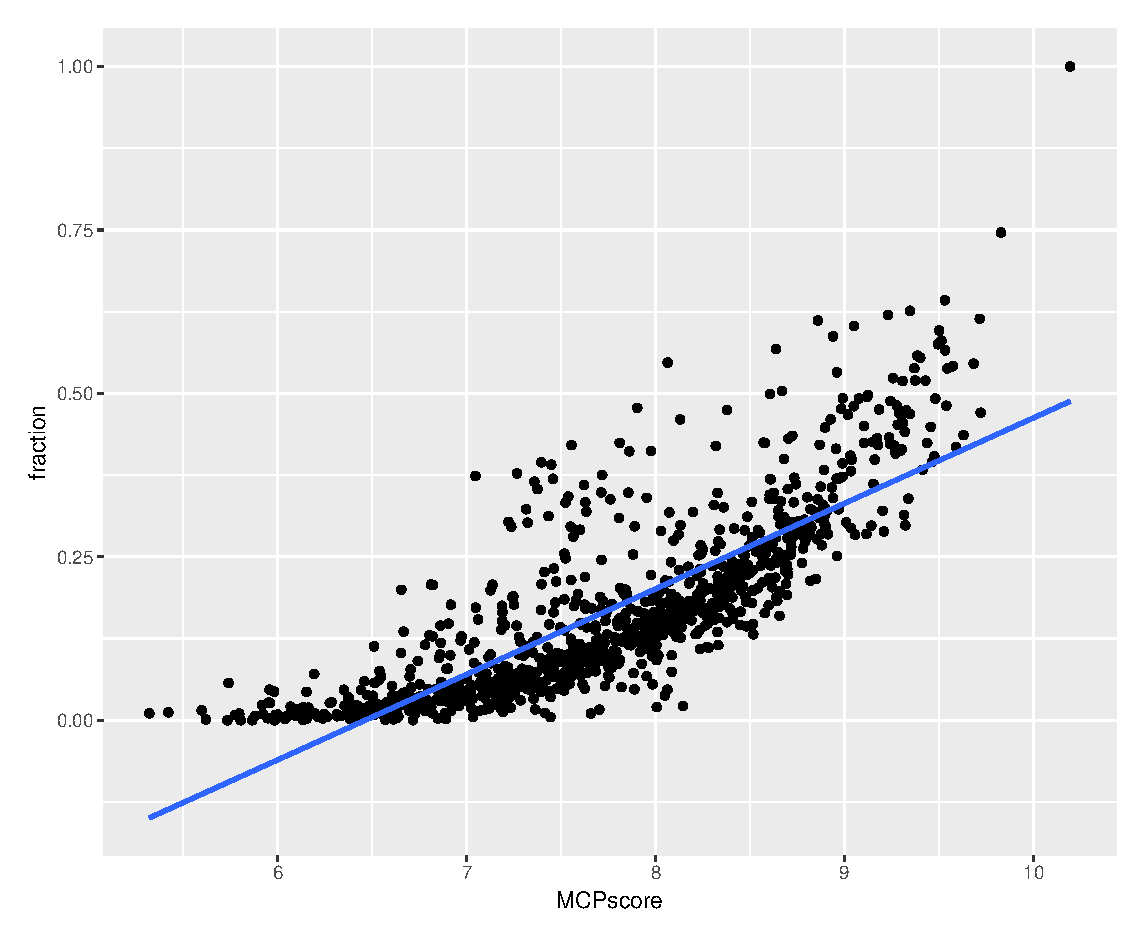
\includegraphics[width=5in]{MCP-B.eps}
     \caption{MCP-count B cell}
     \label{fig:my_label}
 \end{figure}
 \begin{figure}[H]
     \centering
     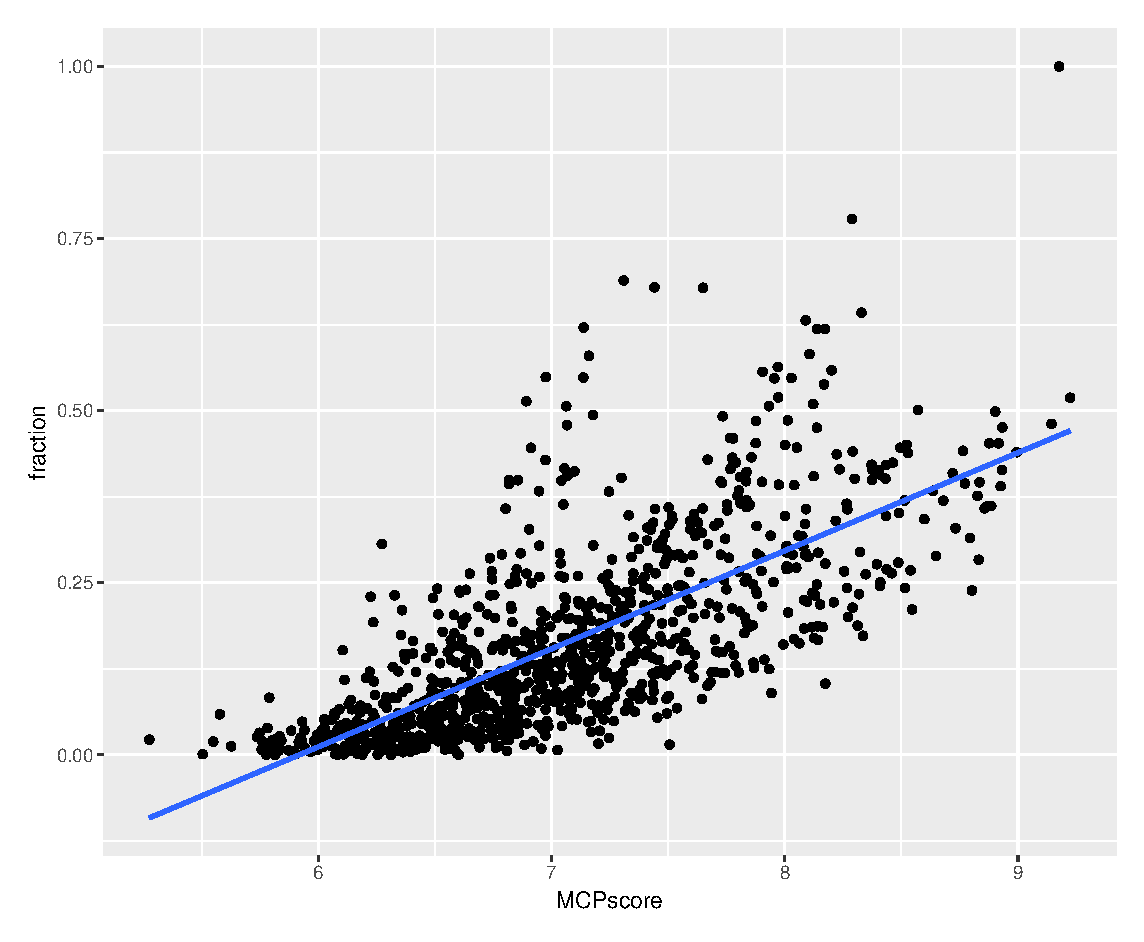
\includegraphics[width=5in]{MCP-NK.eps}
     \caption{MCP-count NK cell}
     \label{fig:my_label}
 \end{figure}
 \begin{figure}[H]
     \centering
     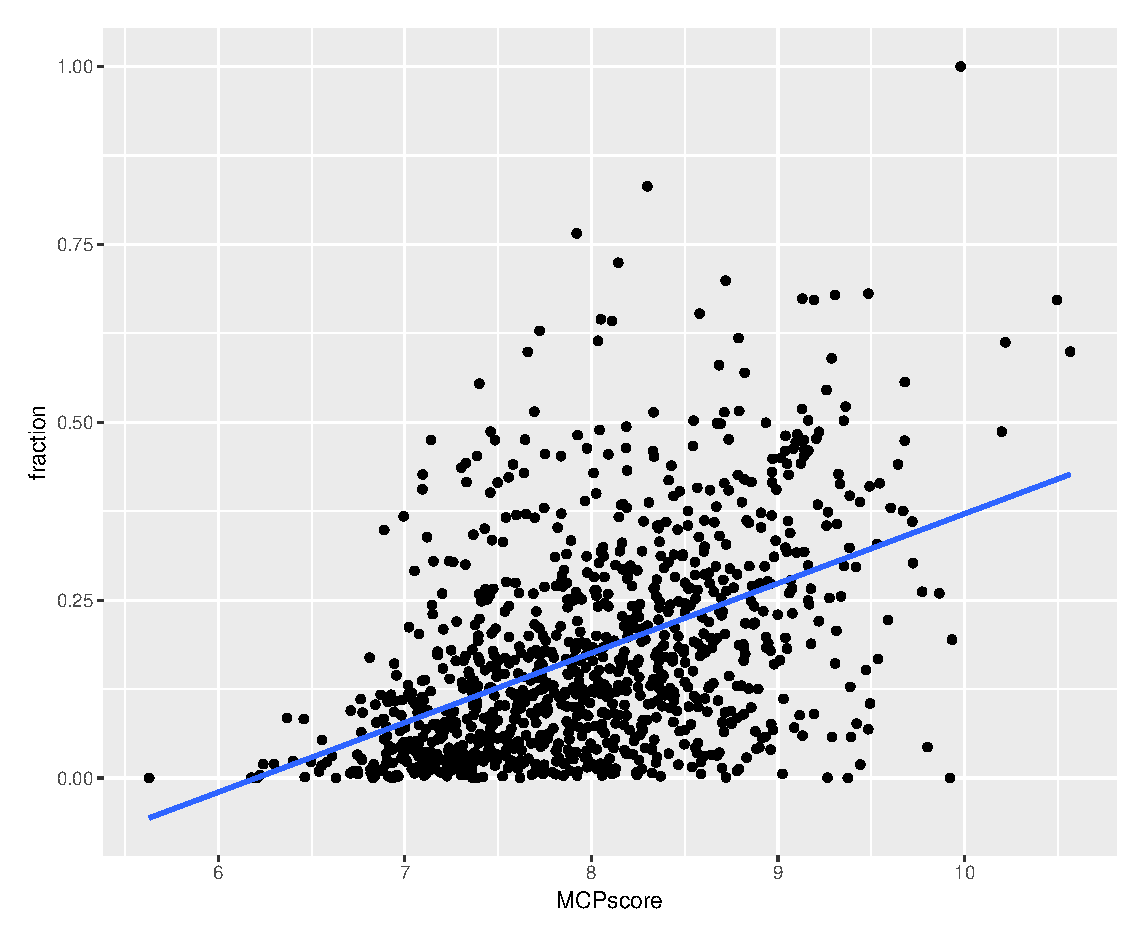
\includegraphics[width=5in]{MCP-MONO.eps}
     \caption{MCP-count Monocytes}
     \label{fig:my_label}
 \end{figure}
\begin{figure}[H]
     \centering
     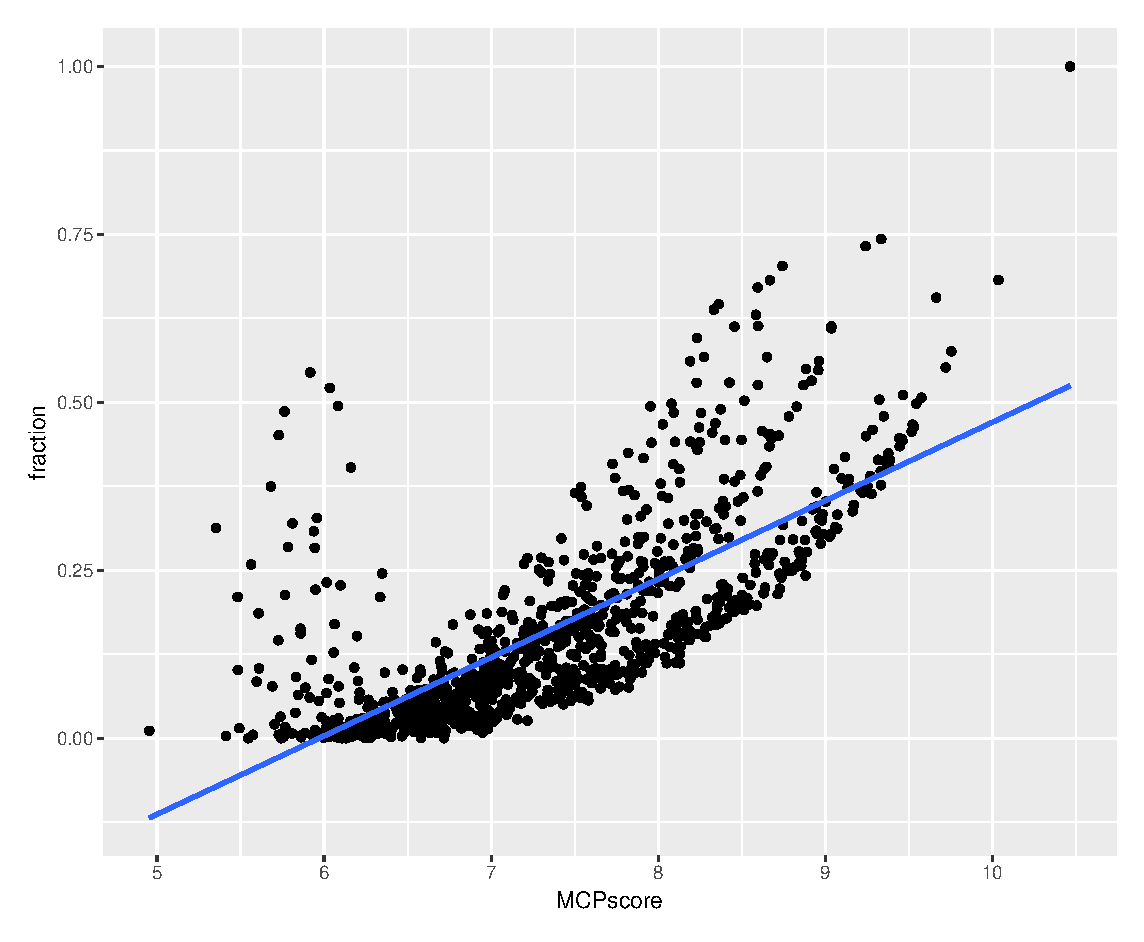
\includegraphics[width=5in]{MCP-NEUT.eps}
     \caption{MCP-count Neutrophils}
     \label{fig:my_label}
\end{figure}
\begin{figure}[H]
     \centering
     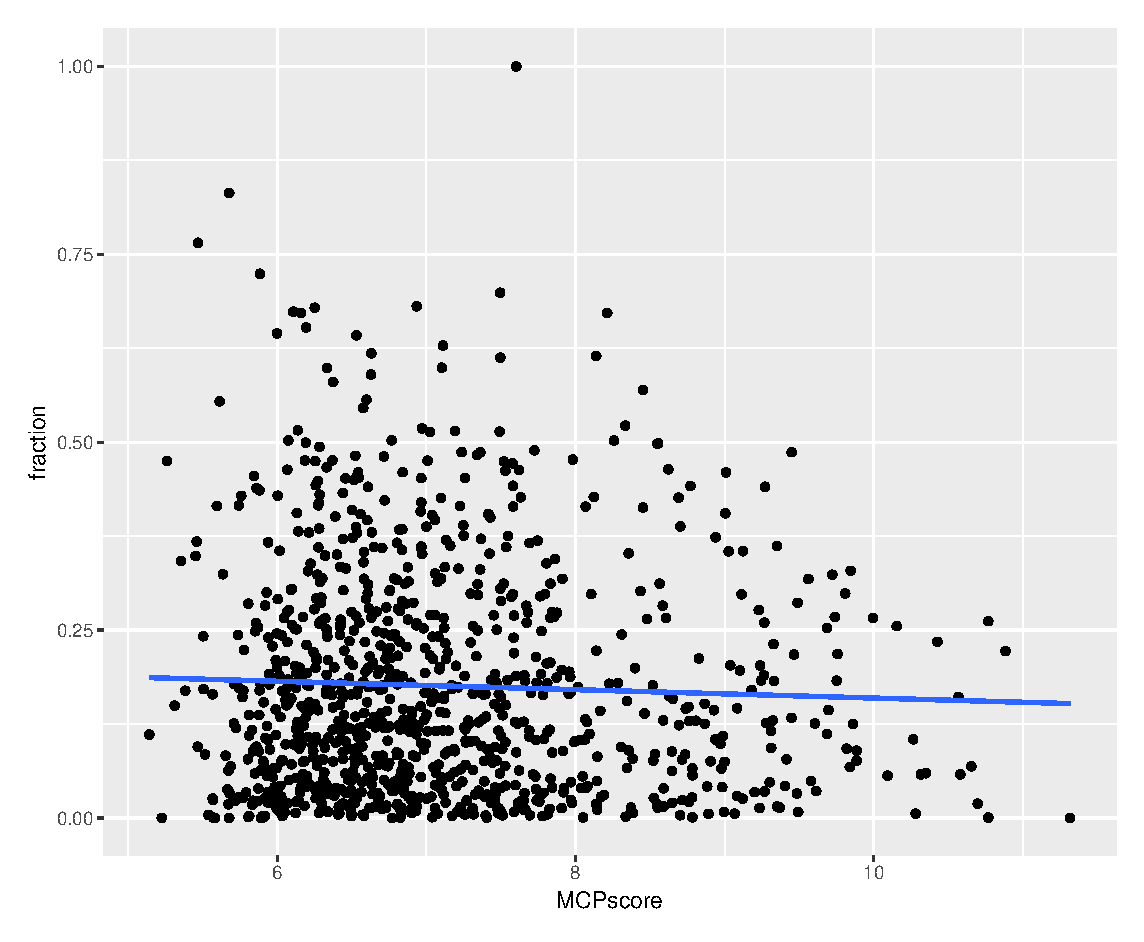
\includegraphics[width=5in]{MCP-MDC.eps}
     \caption{MCP-count Myeloid dendritic cell}
     \label{fig:my_label}
\end{figure}
It can be seen from the experimental results that the correlation between the MCP-count score and the true mixing ratio of the mixed samples is not high, especially Myeloid dendritic cells and Monocytes.
one
\subsection{Mixture availability test}
I got GSE64385 microarray data (including 10 real-time mixed samples of known proportions) from geo. I extracted a given cell type microarray expression data from a purified data set with a consistent ratio of real samples. I verified the availability of the artificial mixture by correlating the expression of the artificial mixture with the actual mixture.
\begin{figure}[H]
     \centering
     \includegraphics[width=5in]{cormixture.png}
     \caption{correlation of expression of artificial mixture and actual mixture}
     \label{fig:my_label}
\end{figure}
It can be seen from the heat map that the correlation between the simulated mixed sample and the real sample is low when the proportion of the sample tumor is high.

\subsection{TCGA Data}
 
\section{Discussions and future work}
List your plan for next week in details. Highlight \todo{important issues} to take note.


(1) implement algorithm.

(2) create signature.

\bibliographystyle{plain}
\bibliography{sample}

\end{document}